\chapter{Organización}
En este apartado se describe cuál ha sido la planificación del proyecto, y cómo 
se ha organizado. Esta planificación se ha desarrollado para poder mantener un
ritmo continuo de desarrollo de tipo ágil, y conseguir un aprovechamiento máximo
del proyecto. Durante el desarrollo de este proyecto se ha realizado paralelamente
pequeños proyectos, por lo que era necesario que se pudiesen observar los resultados
del desarrollo de la forma más inmediata posible. Para ello, como se ha explicado
en el capítulo \ref{cha:metodologia}, se realizan pequeños prototipos de una
funcionalidad que más adelante son integradas en el proyecto.

En la figura \ref{fig:gantt} se presenta un diagrama Gantt en el que se puede observar
las diferentes tareas y fases por las que ha pasado el proyecto, presentando las
correspondientes fechas de inicio y fin que se han estimado durante la ejecución del
proyecto. Al tratarse de un proyecto incremental mediante generación de prototipos,
se han realizado varias iteraciones durante el desarrollo.

Las fases del proyecto se puede dividir en los siguientes bloques:
\begin{itemize}
	\item Recolección de requisitos del sistema y estudio de la tecnología necesaria.
	\item Desarrollo de la Nube de conductores.
	\item Desarrollo de la aplicación para ciclistas.
	\item Desarrollo de la RSU, OBU y HMI.
	\item Verificación del sistema en la calle.
	\item Estudio de los resultados y generar documentación.
\end{itemize}

Los hitos del proyecto son las distintas pruebas que se han hecho de funcionalidades
diferentes del sistema. Durante estas pruebas se analiza el rendimiento que se obtiene
de la comunicación del sistema, se proponen y añaden mejoras que serán incluidas en
siguientes pruebas.

\begin{figure}[t]
	\rotatebox{90} {
		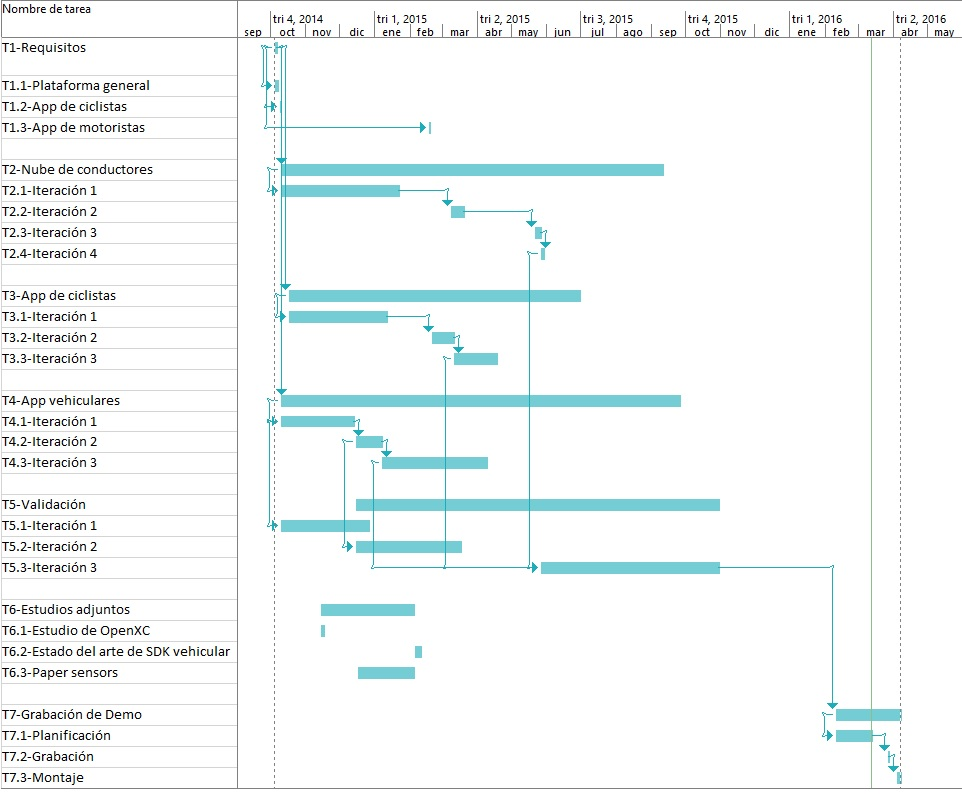
\includegraphics[scale=0.6]{DiagramaGantt}
	}
	\caption{Diagrama de Gantt}
	\label{fig:gantt}
\end{figure}
